\chapter{Learning from ideal data\\}
\label{cha:Learning_algorithm}

This chapter is focussing on the implementation of the inverse reinforcement learning idea that is used to learn the different weights in the comfort cost function $\bm{\theta}^T\bm{F}(\bm{r})$
explained in chapter \ref{cha:Literature_study}. The use of ideal data is assumed which means that vehicle model mismatch is avoided by using the same model for learning the weights as generating the data. Thereby is the approximation that comfort of a driver can be modelled by a simple linear relation of features is exactly for-filled. Data is generated by choosing a set of weights and generating kinematic vehicle signals by the minimization seen in equation \ref{eq:6}. Perfect learning occurs when the chosen weights when generating the data are found back.\\

First the non-linear bicycle model with the used parameters are explained. Further on the concretely used algorithm is discussed. After that a detailed discussion is given about the simulations done in order to check what the algorithm is capable of. The reader must be aware that the learning process discussed, concerns an offline optimization which allows for higher calculations loads because of the absence of binding real time constraints.


\section{Non-linear bicycle model}\label{sec:Vehicle_models}
The free body diagram of the non-linear bicycle model can be seen in figure \ref{fig:bicycle_model}.\\

\begin{figure}[h!]
	\centering
	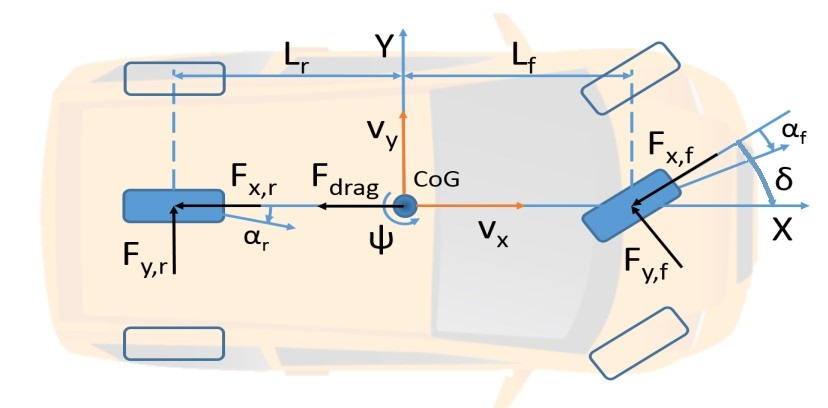
\includegraphics[width=0.5\textwidth]{Bicycle_model_paper.png}
	\caption{Non-linear vehicle bicycle model (Source: \cite{TongDuySon2019}).}
	\label{fig:bicycle_model}
\end{figure}

The model is characterizing the vehicle with 6 states and 2 inputs:
\begin{equation}\label{eq:bicycle_model}
\centering
\bm{X} = 
\begin{bmatrix}
x & y & v_x & v_y & \psi & \dot{\psi}
\end{bmatrix}^{T}
\; and \; \bm{U} = 
\begin{bmatrix}
t_r & \delta
\end{bmatrix}^{T}
\end{equation}

$X$ and $Y$ in the formulation of \ref{eq:bicycle_model} are the position of the centre of gravity of the car in the global coordinate system. $\psi$ is the vehicle yaw angle and $\dot{\psi}$ the yaw angular velocity. $v_x$ and $v_y$ are the vehicle velocities in the local vehicle frame. The input vector consists of the throttle control input $t_r$ and the steering angle $\delta$.\\

The equations of motion \cite{TongDuySon2019} are:
\begin{equation}\label{eq:bicycle_model_eqmotion}
\begin{aligned}
\dot{x} = v_x cos(\psi) - v_y sin(\psi)\\
\dot{y} = v_x sin(\psi) + v_y cos(\psi)\\
\dot{\psi} = \dot{\psi}\\
m \dot{v}_x = F_{x,f} cos(\delta) - F_{y,f} sin(\delta) + F_{x,r} - F_{drag} + m v_y \dot{\psi}\\
m \dot{v}_y = F_{x,f} sin(\delta) + F_{y,f} cos(\delta) + F_{y,r} - m v_x \dot{\psi}\\
I_z \ddot{\psi} = L_f (F_{y,f} cos(\delta) + F_{x,f} sin(\delta)) - L_r F_{y,r}
\end{aligned}
\end{equation}

The drag force is calculated as:
\begin{equation}\label{eq:bicycle_Fdrag}
\begin{aligned}
F_{drag} = C_{r0} + C_{r1} v_x^2
\end{aligned}
\end{equation},
with $C_{r0}$ the roll resistance and $C_{r1}$ the air drag contributions.\\

To calculate the tyre forces, a linear tyre model is used instead of a more complex non-linear model e.g. Pacejka tire model. The longitudinal tyre forces are calculated as:
\begin{equation}\label{eq:bicycle_Fx}
\begin{aligned}
F_{x,f} = \frac{t_r T_{max}}{2 R_w}\\
F_{x,r} = F_{x, f}
\end{aligned}
\end{equation}

$R_w$ is the wheel radius and $T_{max}$ a measure for the maximum torque the engine is able to supply. In this way, four wheel drive is assumed and the total torque is equally distributed between front and rear axle (division by 2 in above equations). The coefficient $t_r$ is the normalised wheel torque and can have a value between -1 and 1 (negative for braking).
The lateral tyre forces are calculated based on the tyre slipangles $\alpha_f$ and $\alpha_r$:
\begin{equation}\label{eq:bicycle_slipangle}
\begin{aligned}
\alpha_f = -atan(\frac{\dot{\psi} L_f + v_y}{v_x}) + \delta\\
\alpha_r = atan(\frac{\dot{\psi} L_r - v_y}{v_x})
\end{aligned}
\end{equation},
resulting in:
\begin{equation}\label{eq:bicycle_Fy}
\begin{aligned}
F_{y,f} = 2 K_f \alpha_f\\
F_{y,r} = 2 K_r \alpha_r
\end{aligned}
\end{equation}\\
The use of this linearised lateral tyre model is valid for small lateral accelerations ($a_y <= 4 m/s^2$) and slip angles ($\alpha <= 5^o$) \cite{TongDuySon2019}. It is acceptable to use this approximation model in this thesis as the goal is learn a comfortable and thus smooth manoeuvre e.g lane change. These constraints will also be checked during the validation in Chapter \ref{cha:Validation}.\\

The fixed model parameter used during the simulations are given in table \ref{table:vehicel_model_param}. These correspond to common used vehicle parameters as provide by Siemens Digital Industries Software - NVH R\&D engineering department.

\begin{table}[h]
	\centering
	\begin{tabular}{|p{5cm}|p{2cm}|}
		\hline
		\textbf{Parameter} & \textbf{Value}\\ \hline		
		Vehicle mass $m$ [kg] & 1430\\ \hline
		Moment of inertia $I_z$ [$kgm^2$] & 1300\\ \hline
		Front axle distance $L_f$ [m] & 1.056\\ \hline
		Rear axle distance $L_r$ [m] & 1.344\\ \hline
		Roll resistance coefficient $C_{r0}$ [N] & 0.6\\ \hline
		Air drag coefficient $C_{r1}$ [$\frac{Ns^2}{m^2}$] & 0.1\\ \hline
		Engine torque limit $T_{max}$ [Nm] & 584\\ \hline
		Wheel radius $R_w$ [m] & 0.292\\ \hline
		Lateral front tyre stiffness $K_{f}$ [N] & 41850.85\\ \hline
		Lateral rear tyre stiffness $K_{r}$ [N] & 51175.78\\ \hline
		
	\end{tabular}
	\caption{Used vehicle model parameters.}
	\label{table:vehicel_model_param}
\end{table}

\section{Formulation of the algorithm}
The goal of the learning algorithm is to learn the weights $\bm{\theta}$ in the pre-defined comfort objective function: $\bm{\theta}^T\bm{F}(\bm{r})$. The features that are the entries of the feature vector $\bm{F}(\bm{r})$ have to capture a notion of comfort felled by the driver. Based on the literature study conducted in Chapter \ref{cha:Literature_study} and paper \cite{Kuderer2015a}, the amount of discomfort can be modelled by following features during timespan $T$ of the maneuver. The scenario of a lane change on a highway is chosen. Further in this thesis a validation of the method is done by also looking into a longitudinal acceleration maneuver. $T$ itself is aside of the state and control variables of the non-linear bicycle model also an optimization variable during the learning process.The simulations done in this thesis were performed on a notebook with Intel Core i7-7920HQ CPU @ 3.10GHz and 32 GB of RAM memory.\\


\subsection{Flow of the algorithm}
The best weights are found when the paths that are generated with the comfort cost function \ref{eq:CC} explain the observed path best. Similarity between the observed path and the one that follows from minimizing the objective \ref{eq:CC} is quantitated  by the difference between the feature values of the observed path and the obtained one. The flow of the single data set learning algorithm can be seen in Figure \ref{fig:basic learning}.

\begin{figure}[h!]
	\centering
	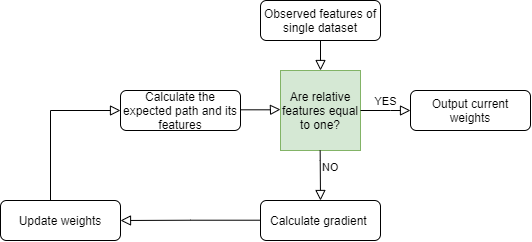
\includegraphics[width=1.0\textwidth]{basic_learning.png}
	\caption{Basic flow of the reinforced learning algorithm.}
	\label{fig:basic learning}
\end{figure}

The learning is started by guessing a set of weights e.g. all equal to one. Equation \ref{eq:CC} is minimized in order to generate an expected path for these weights. From this calculated path, features can be retrieved from where relative features $f_{rel,i}$ are calculated by dividing the calculated features by the features that are derived of the observed path. A perfect match is acquired when the division equals one. The tolerance on convergence towards one, is chosen during this chapter equal to $10^{-4}$.  When obtained, the learning algorithm is stopped and the learned weights are outputted.\\

While no convergence takes place the weights are updated, making use of the RPROP algorithm explained in Chapter \ref{cha:Literature_study}. In order to apply the RPROP method only the sign of the gradient is needed, because the size of the step $\alpha$ is decoupled of the size of the gradient. Because the gradient is given by $\pdv{\bm{F}}{\bm{\theta}} = \bm{F}_{obs} - \bm{F}(\bm{r}_{expected})$  and the update of the weight is achieved by applying the gradient method according to $\bm{\theta}^{k+1} = \bm{\theta}^{k} - \alpha \pdv{\bm{F}}{\bm{\theta}}^k $, the weight $\theta_i$ is decreased if $f_{obs,i}>f_{i}(\bm{r_{exptected}})$ and increased when $f_{obs,i}<f_{i}(\bm{r}_{exptected})$. The optimization with fixed weights that is solved during each iteration in order to calculate the expected path, which equals the most comfortable path, can be seen in optimization \ref{opt:basic_opti_w}. \\

\begin{equation}\label{opt:basic_opti_w}
\begin{aligned}
\min_{\bm{X}(.),\bm{U}(.), T} \quad & \sum_{k = 0}^{N-1} \bm{\theta}^T\bm{F}(\bm{X}^k,\bm{U}^k, T) \\
\textrm{s.t.} \quad & \bm{X}^{k+1} = I(\bm{X}^{k}, \bm{U}^{k}) & k = [0,\cdots, N-1]\\
& \bm{X}^{0}= \bm{X}_{intitial} \\
& \bm{G}(\bm{X}^{k},\bm{U}^{k}) \geq 0	& k = [0,\cdots, N]\\
& \bm{H}(\bm{X}^{k},\bm{U}^{k}) = 0	& k = [0,\cdots, N]\\
& \bm{X}^{k}\in \mathbb{R}^{6x1}  & k = [0,\cdots, N]\\
& \bm{U}^{k}\in \mathbb{R}^{2x1} \hspace{3 mm} & k = [0,\cdots, N-1]\\
& T \in \mathbb{R},\hspace{3 mm} N,i,l \in \mathbb{N}
\end{aligned}
\end{equation}

Where $\bm{X} \in \mathbb{R}^{6xN+1}$ and $\bm{U}\in \mathbb{R}^{2xN}$ contain respectively the states and controls  \ref{eq:bicycle_model} during the maneuver, complemented with the time of the maneuver $T$. In order to discretize time a multiple shooting is adopted as is explained in section \ref{s:time_dis} The amount of integration intervals $N$ chosen in this chapter is equal to $500$ and equals the amount of control intervals in order to go from the initial state towards the end state. Taken into account that a lane change maneuver modelled takes around $6$ seconds, a sampling time around $100 \hspace{1mm} \frac{samples}{s}$ is obtained with $N$ taken equal to $500$. Inside the function $I$ the Runge-Kutta time integration method is embedded in order to connect different states over time when a certain control is applied for $\Delta T$. The path constraint vector $\bm{G} \in \mathbb{R}^{Lx1}$ demarcate together with the equality constraint vector $\bm{H} \in \mathbb{R}^{Qx1}$ the feasible area of the solutions for $\bm{X}$, $\bm{U}$ and $T$. An overview of $\bm{G}$ and $\bm{H}$ used can be found by equation \ref{eq:G} and \ref{eq:H}.



\begin{equation}\label{eq:G}
\bm{G} =
\begin{Bmatrix}
-1 \leq t_r^k \leq 1, & k = [0,\cdots, N-1] \\
-\frac{Width\hspace{1mm}Road}{2} \leq y^k \leq \frac{3\cdot Width\hspace{1mm}Road}{2}, & k = [0,\cdots, N] \\
x^k \geq 0, & k = [0,\cdots, N] \\

\end{Bmatrix}
\end{equation}\\

It should be noted that the physical limits of the vehicle so as maximum accelerations, velocities are not taken into account. This is done because they were not bounding during a comfortable lane change maneuver and thus are not influencing the optimal solution. Ofcourse when the learning is applied in a more general scenario these constraints should be included in order to get a more robust optimization formulation.

\begin{equation}\label{eq:H}
\bm{H} =
\begin{Bmatrix}
y^N = Width\hspace{1mm}Road \\ \vspace{1mm}
vy^N = 0 \\\vspace{1mm}
ay^N = 0 \\\vspace{1mm}
\psi^N = 0 \\\vspace{1mm}
\dot{\psi}^N = 0 \\\vspace{1mm}
a_{t,y}^N = 0 \\\vspace{1mm}
j_y^N = 0 \\\vspace{1mm}
a_{t,y}^0 = 0 \\\vspace{1mm}
j_y^0 = 0 
\end{Bmatrix}
\end{equation}\\

These constraints displayed in $\bm{H}$ make sure that initial state of the vehicle is just before the start of the lane change and the last state of the vehicle is when the lane change maneuver is completely finished. The initial state $\bm{X}_{intitial}$ as stated by optimization \ref{opt:basic_opti_w} can be seen in \ref{eq:X0}.
\begin{equation}\label{eq:X0}
\bm{X}_{initial} =
\begin{bmatrix}
 0\\ 
 0\\
 v_{start}\\
 0\\
 0\\
 0\\
\end{bmatrix}
\end{equation}\\

From this formulation it is clear that when the generation of ideal observation data by solving \ref{opt:basic_opti_w} for a set of manually chosen weights (Section \ref{s:GD}), changing the parameters $v_{start}$ and $Width \hspace{1mm}Road$ will lead to different lane change maneuvers.\\ The initial guess used in \ref{opt:basic_opti_w} for $\bm{X}, \bm{U} \;and\; T$ during the learning process are extracted from the observation. 
\subsection{Objective function}\label{s:obj}

\begin{equation}\label{eq:obj}
discomfort = \theta_1 \cdot f_1 +\theta_2 \cdot f_2 +\theta_3 \cdot f_3 +\theta_4 \cdot f_4 +\theta_5 \cdot f_5 \\
\end{equation}
\[	f_i, \theta_i \in \mathbb{R} \hspace{5mm}
i \in \mathbb{N}\]\\


\textit{Feature 1: longitudinal acceleration}
\begin{equation}\label{eq:flong_acc}
f_{1}:\bm{r}\xrightarrow{}f_1(\bm{r})=\int_{0}^{T}a_{x,total}^{2}(t) dt
\end{equation}
Feature one is assessing the amount of discomfort by integrating the total longitudinal acceleration in the local axis fixed to the vehicle as can be seen in Figure \ref{fig:bicycle_model}. The total longitudinal acceleration  $a_{x,total} $ is the sum of the tangential acceleration $ a_{x,tangential}$ and the normal acceleration $a_{x,normal}$. These 2 variables can respectively be linked to the optimization variables regarding the vehicle model of equation \ref{eq:bicycle_model} by $\pdv[2]{v_x}{t}$ and $-v_y\cdot\dot{\psi}$. By including the normal acceleration, the centripetal force and hence the curvature of the path is taken into account. \\ 

\textit{Feature 2: lateral acceleration}
\begin{equation}\label{eq:flat_acc}
f_{2}:\bm{r}\xrightarrow{}f_2(\bm{r})=\int_{0}^{T}a_{y,total}^{2}(t) dt
\end{equation}
Feature two is assessing the amount of discomfort by integrating the total lateral acceleration in the local axis while assuming a straight road. The total lateral acceleration  $a_{y,total} $ is the sum of the tangential acceleration $ a_{y,tangential}$ and the normal acceleration $a_{y,normal}$. These 2 variables can respectively be linked to the optimization variables regarding the vehicle model of equation \ref{eq:bicycle_model} by $\pdv[2]{v_y}{t}$ and $v_x\cdot\dot{\psi}$.\\

\textit{Feature 3: lateral jerk}
\begin{equation}\label{eq:flat_jerk}
f_{3}:\bm{r}\xrightarrow{}f_3(\bm{r})=\int_{0}^{T}j_y^{2}(t) dt
\end{equation}
Feature three is assessing the amount of comfort by integrating the total change of acceleration during the followed path. \\

\textit{Feature 4: desired speed}
\begin{equation}\label{eq:des_speed}
f_{4}:\bm{r}\xrightarrow{}f_4(\bm{r})=\int_{0}^{T}(v_{des}-v_x)^2 dt
\end{equation}
$v_{des}$ is assumed to be a constant value in this paper and set equal to start velocity just before starting the lane change.\\

\textit{Feature 5: desired lane change}
\begin{equation}\label{eq:des_lane_change}
f_{5}:\bm{r}\xrightarrow{}f_5(\bm{r})=\int_{0}^{T}(y_{lane\_change}-y)^2 dt
\end{equation}
$y_{des}$ is a constant and is the desired lateral distance completed after the lane change. If the goal is faster achieved, this is interpreted as comfort for the driver.
\\

In order to implement the above defined first and second derivative and integrations in a CasADi optimization environment, discretization with a numerical scheme is needed. The first and second derivative are discretized by means of a central scheme as can be seen in equation \ref{eq:CC}


\begin{subequations}\label{eq:CC}
	\begin{equation}
	\pdv{\phi}{t} = \frac{\phi(i+1)-\phi(i-1)}{2\Delta t}
	\end{equation}
	\begin{equation}
	\pdv[2]{\phi}{t} = \frac{\phi(i+1)\phi(i)+\phi(i-1)}{\Delta t^2}
	\end{equation}
\end{subequations}

The Crank-Nicolson numerical integration as is displayed in equation \ref{eq:CN} is used in order to obtain the different feature values of feature $i$.
\begin{subequations}\label{eq:CN}
	\begin{equation}
	\int_{f_i(t^n)}^{f_i(t^{n+1})}df_i=\int_{t^n}^{t^{n+1}} I(t) \cdot dt	
	\end{equation}
	\begin{equation}
	f_i^{n+1} -f_i^{n} = \frac{1}{2}\frac{I(t^{n+1})+I(t^n)}{\Delta t}
	\end{equation}
\end{subequations}\\

The objectives seen in equation \ref{eq:CC}, that consists out of a set of comfort features models the amount of discomfort experienced during a maneuver by mapping 2D kinematic signals onto a scalar feature values. By finding the driver specific weights in \ref{eq:CC} it is possible to model driver preferences between different comfort features. With this information an autonomous vehicle can perform path planning of the most comfortable path to do a maneuver.  As is shortly discussed in Chapter \ref{cha:Literature_study}, the perception of save driving by the autonomous vehicle contributes to the amount of comfort that will be experienced during driving. Because this thesis is focussing on the development and validation of a reinforcement learning algorithm, the environment is not taken into account. However this can easily be done if data of the state of other vehicles is available by modelling the distances between different vehicles by equation \ref{eq:comfort_feature} as suggested in \cite{Kuderer2015a}. 

\begin{equation}\label{eq:comfort_feature}
f_d= \sum_{k = 1}^{L}\int_{0}^{T}\frac{1}{(x_{o,k}(t)-x)^2+(y_{o,k}(t)-y)^2}\cdot dt
\end{equation}
\[L \in \mathbb{N}\]

With $[x_o,y_o]_k$ the position of a different vehicle and $L$ the total amount of vehicles in the nearby area.\\

Not only the bird's eye view distance between two different vehicles plays a role, but also the following distance of the vehicle in front in the same lane is important. This can be modelled as suggested by \cite{Kuderer2015a} by:  

\begin{equation}\label{eq:lane_d}
f_d= \int_{0}^{T} max(0,\hat{d}-d(t))\cdot dt
\end{equation}

In equation \ref{eq:lane_d}, $\hat{d}$ is the desired distance and $d(t)$ is the distance between the vehicle in front in the current lane.\\


An other assumption that not is discussed in this thesis is the time limit to finish a maneuver. In a real life application however this limit often influence the maneuver. After the weights are identified, the most comfortable path in a limited time span can be calculated for a specific driver. If no time limit serves as bottleneck, the time of the maneuver can be included as optimization variable and long and smooth lane changes are planned. 

\subsection{Normalization factors and initialization} \label{s:norm}
In order to nullify the effect of order of size given by the units in the objective discussed in section \ref{s:obj}, a normalization of the features is used. The kinematic signals of an example lane change are produced and the same features that are used in the objective function are calculated from it. These will be the normalization factors. Then the objective function is divided by the corresponding normalization factor which means that a feature that inherently gives a small feature values, will be divided by a small value and the other way around, an inherently large feature value will be divided by a large value. In this thesis the example lane change is produced as is described in section \ref{s:GD} with weights equal to $ \bigl[ \begin{smallmatrix} 4,&5,&6,&1,&2\end{smallmatrix}\bigr]$ and corresponding to the objective function of section \ref{s:obj} and making use of normalization factors and an initial guess provided by data of a lane change that was available at Siemens. Table \ref{table:norm} gives an overview of the lane change normalization factors used in this chapter. 

\begin{table}[h!]\label{table:norm}
  \centering
  \begin{tabular}{@{}lr@{}} 
    Normalization factor    & Value\\ \midrule
    Nr.1      & 0.0073\\
    Nr.2          & 2.64\\
    Nr.3       & 11.28\\
    Nr.4       & 0.047\\
    Nr.5  & 17.14\\ \bottomrule
  \end{tabular}
  \caption{Overview of  normalization factors.}
\end{table}

The solver used to calculate the states and control signals in \ref{opt:basic_opti_w} is the interior point solver IPOPT which is open source code. The idea behind the solver is to smoothing the KKT conditions and transform it to a smooth root finding problem. \cite{Panos_opti} Because IPOPT is a interior boundary method, a feasible initial guess is needed.\\
Every time that the expected path has to be calculated as is visualised in flow diagram \ref{fig:basic learning}, the optimization \ref{opt:basic_opti_w} is performed with as initial guess the observed maneuver.\\

\subsection{Ideal data generation} \label{s:GD}
As mentioned above the term 'ideal data' concerns data that is generated with a non-linear bicycle model and exactly fulfils the assumption that the observations are minimizing an underlying discomfort function. More over the discomfort function is the same as the one used in the learning algorithm and this means that the generated path is a the solution of the objective function discussed in section \ref{s:obj} for weights $\bm{\theta}$ chosen in advance. Because that the observations are exactly representing the comfort function in the learning algorithm and the absence of vehicle model mismatch, weights can be learned that perfectly explain the observations. This is translated in a accurate matching of the feature values discussed in \ref{s:obj}. Because beforehand it is know what the weights should be in \ref{eq:obj}, the ideal data can serve as a validation of the developed learning algorithm.\\

The relative weights chosen are $ \bigl[ \begin{smallmatrix} 4,&5,&6,&1,&2\end{smallmatrix}\bigr]$, which gives as absolute weights  $ \bigl[ \begin{smallmatrix} 549.63, &1.90, &0.53,  &21.43, &0.12\end{smallmatrix}\bigr]$ when the normalization of \ref{s:norm} is taken into account. The objective that is used in \ref{opt:basic_opti_w} and outputs the ideal data is given by \ref{eq:obj_ideal_data}.

\begin{equation}\label{eq:obj_ideal_data}
discomfort = \frac{4}{0.0073} \cdot f_1 +\frac{5}{2.64} \cdot f_2 +\frac{6}{11.28} \cdot f_3 +\frac{1}{0.047} \cdot f_4 +\frac{2}{17.14} \cdot f_5 \\
\end{equation}
\[	f_i \in \mathbb{R}, \hspace{1mm}
i \in \mathbb{N}\]\\

Because of the normalization the relative weights will quantify the trade-offs between different comfort features without the disturbance of units used. Aside of this it allows to learn weights faster because of the absence of big size differences that are present in absolute weights. When multiple ideal data sets have to be generated in order to serve as observations, the initial speed and width of the lateral distance \\
In order to determine if the generated data is a local solution of the optimization of \ref{opt:basic_opti_w}, three different initial guesses are used. From which two were coming from example lane changes produced by the 15 dof Amesim vehicle model of Siemens and the other one was a generated path with all weights equal to one and using Siemens dataset 1 as initial guess. Figure \ref{fig:IG} shows the three initial guesses used. It could be concluded that the three guesses gave the same generated signals for all states and controls of the non-linear bicycle model. Figure \ref{fig:result_GD} shows the three generated paths which lay exactly on each other. Further on in this chapter the intitial guess is set equal to the observed data.

\begin{figure}[h!]
	\centering
	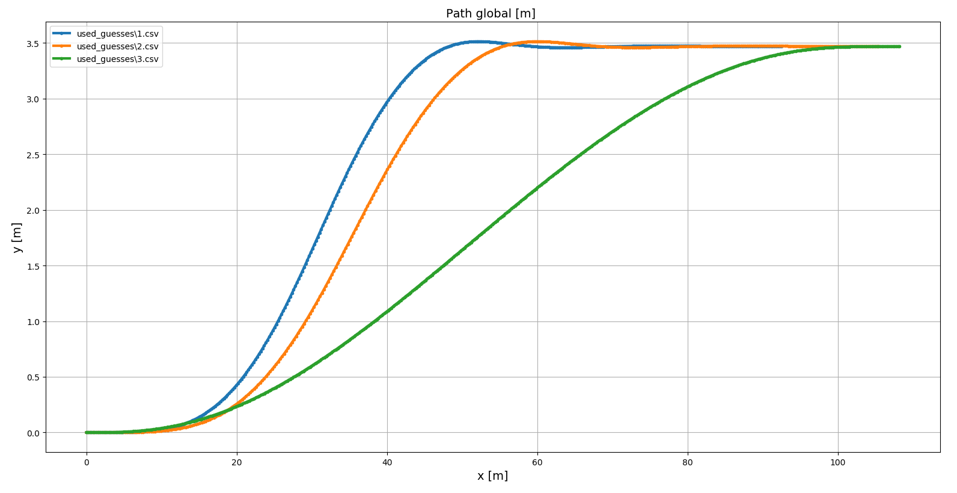
\includegraphics[width=1.0\textwidth]{IG.png}
	\caption{Different initial guesses used in \ref{opt:basic_opti_w} to generate data.}
	\label{fig:IG}
\end{figure}

\begin{figure}[h!]
	\centering
	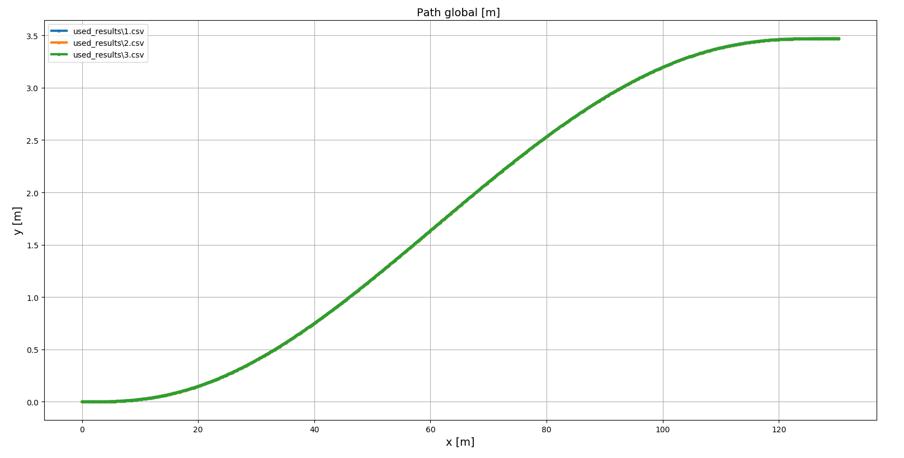
\includegraphics[width=1.0\textwidth]{result_GD.png}
	\caption{Different ideal data paths generated with \ref{opt:basic_opti_w}.}
	\label{fig:result_GD}
\end{figure}

\section{Ideal data learning results}
This section discusses the results from using the learning algorithm on generated ideal data which is generated making use of the above discussed normalization values in combination with relative chosen weights of $ \bigl[ \begin{smallmatrix} 4,&5,&6,&1,&2\end{smallmatrix}\bigr]$. The first simulation discusses the learning of three datasets that are generated with the same chosen weights. The different datasets are A $(V_0:22.22\hspace{1mm}\frac{m}{s},\hspace{1mm} L:3.47\hspace{1mm}m)$, dataset B $(V_0:22.22\hspace{1mm}\frac{m}{s},\hspace{1mm} L:6.94\hspace{1mm}m)$ and dataset C $(V_0:25.00\hspace{1mm}\frac{m}{s},\hspace{1mm} L:3.47\hspace{1mm}m)$. The convergence criteria to stop the learning algorithm displayed in Figure \ref{fig:basic learning} is when the maximum amount of iterations equal to $300$ is reached or if the feature values which use the learned weight match accurately the ones of the observed data according to following formula $f_{rel,i} = \frac{f_{calc,i}}{f_{obs,i}} \leq 10^{-4}$.

\subsection{Sequential learning}
In this section dataset A is learned followed by dataset B and as last dataset C.
As initial guess of the weights $\bigl[ \begin{smallmatrix} 1.0,&1.0,&1.0,&1.0,&1.0\end{smallmatrix}\bigr]$ is used.  The resulting paths can be seen in Figure \ref{fig:result_seq} and Figure \ref{fig:convergence_seq} gives the convergence of $f_{rel,i}$ towards one.\\

\begin{figure}[h!]
	\centering
	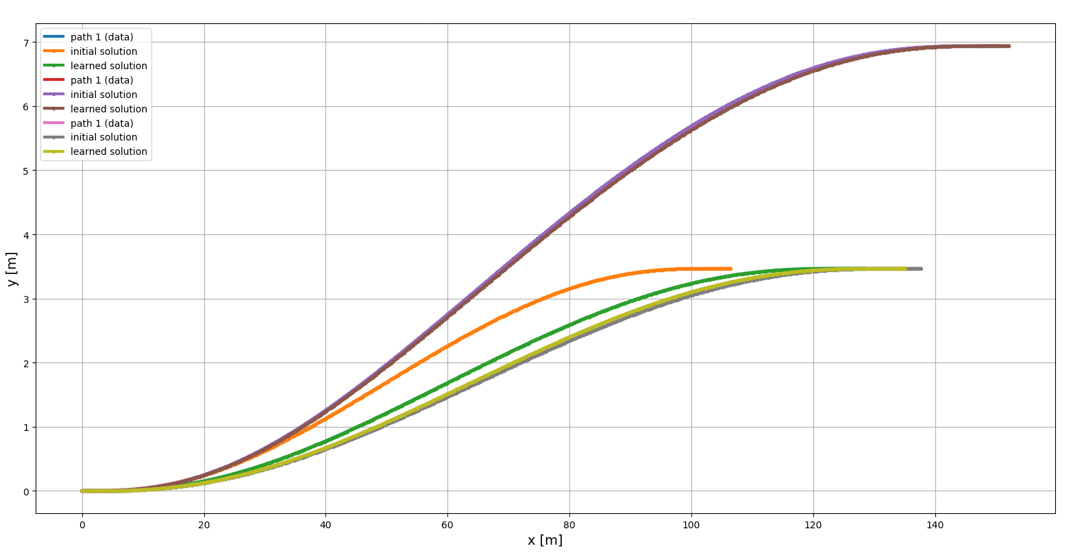
\includegraphics[width=1.0\textwidth]{result_seq.png}
	\caption{Overview of initial guesses, learned and observed trajectories.} 
	\label{fig:result_seq}
\end{figure}

\begin{figure}[h!]
	\centering
	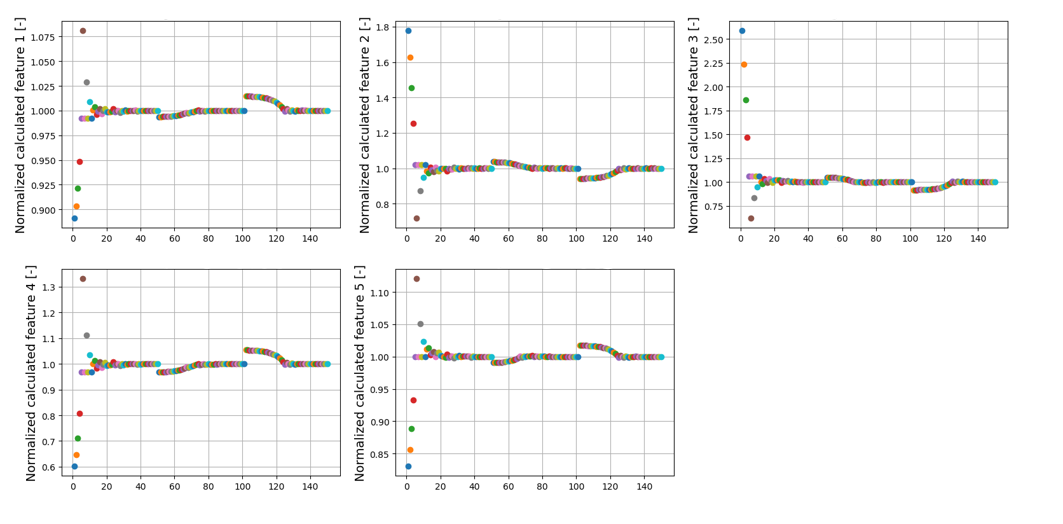
\includegraphics[width=1.2\textwidth]{convergence_seq.png}
	\caption{Convergence of the features with learned weights towards the observed features according to section \ref{s:obj}}
	\label{fig:convergence_seq}
\end{figure}

Convergence is attained after $50$, $51$ and $49$ iterations. From Figure \ref{fig:result_seq} it is clear that when features accurately match as visualized in Figure \ref{fig:convergence_seq}, the observed path is accurately reconstructed when using ideal observations. It can be concluded that fitting of the features gives a good reproduction of the individual state and control signals. Furthermore convergence is fast obtained because the amount of iterations stays limited and simulation time is under 5 minutes per dataset.\\

 An interesting result however is that the corresponding features are not found back. The learned weights are respectively $\bigl[ \begin{smallmatrix} 0.45  ,&1.44 ,&1.68 ,&0.39,&0.60\end{smallmatrix}\bigr]$, 
 
 $\bigl[ \begin{smallmatrix} 0.45  ,&1.48 ,&1.71 ,&0.35,&0.59\end{smallmatrix}\bigr]$ and $\bigl[ \begin{smallmatrix} 0.63  ,&1.43 ,&1.69 ,&0.37,&0.60\end{smallmatrix}\bigr]$. This is visualized in Figure \ref{fig:convergence_seq} by the small jump when switched to a different dataset. Figure \ref{fig:result_seq} shows in orange the first initial guess and in green the learned solution which matches the observed one in blue. The other generated paths start from a close but not perfect initial guess.\\
 
 For each different dataset features match exactly but this is not done for the exact same weights because local solutions exist that explain individual datasets. It should be noted that the relative sizes of the learned weights matches the original one except for the feature concerning longitudinal acceleration which don't play a dominant role during a lane change. \textbf{Question: how is this when you do an acceleration maneuver??}\\
 
 Next the influence of the numerical discretization is checked. A better discretization is obtained when a larger amount of optimization points $N$ is chosen which lead to a smaller time discretization $dt$, but comes at the cost of a higher computational load. Figure \ref{fig:N_influence} shows the error on the features discussed in section \ref{s:obj} when using the learned weights based on dataset A for predicting the observations of dataset B. The convergence criteria of the learned weights are set on $f_{rel,i}$ equal to $10^{-1}$. It is concluded that there is no large influence on the amount of optimization points chosen.\\
 
 \begin{figure}[h!]
 	\centering
 	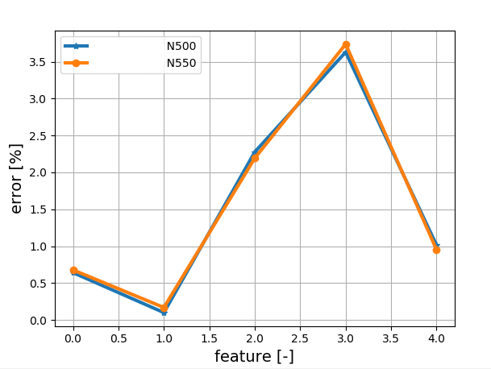
\includegraphics[width=0.7\textwidth]{N_influence.png}
 	\caption{Different error made when using a different amount of optimization points in \ref{opt:basic_opti_w}.}
 	\label{fig:N_influence}
 \end{figure}
 
 In order to further validate the learning algorithm, the chosen weights were given as initial guess making use of one dataset in order to check if it would diverge from the ideal global solution. As expected the algorithm converged after the first iteration. Next a guess close to the global solution was tried. The algorithm converged after $41$ iterations and outputted $\bigl[ \begin{smallmatrix} 4.01,&5.29,&6.33,&1.09,&2.12\end{smallmatrix}\bigr]$ and not $\bigl[ \begin{smallmatrix} 4.0,&5.0,&6.0,&1.0,&2.0\end{smallmatrix}\bigr]$ which proofs that a lot of local solutions exist.\\  
 
 From above tests it can be concluded that the local solutions of individual datasets do not match and that the amount of mismatch has only a small dependants on the amount of optimization points. The next step to take is to combine different datasets in simultaneous learning instead of sequential learning in order to try to converge to weights that predict best for multiple datasets. 
 
 \subsection{Conflict method}
 The first method proposed is the conflict method. Is main idea is to update the weights in the common direction of the gradient seen in equation \ref{eq:new} of the different datasets. If the direction of update according to gradient method is conflicting between different datasets the update of the weight in question is put on hold. The updating will be resumed when the conflict is resolved by updating the other weights. This is possible because the features are not independent of each other. Figure \ref{fig:conflict} shows how the conflict method will be embedded in the basic flow of the learning algorithm.\\
 
  \begin{figure}[h!]
 	\centering
 	\includegraphics[width=1.25\textwidth]{conflict.png}
 	\caption{Flow of the conflict method as part of the basic flow diagram of Figure \ref{fig:basic learning}}
 	\label{fig:conflict}
 \end{figure}

Depending if the previous case in the RPROP algorithm was case 2 and the sign difference between the current and previous gradient, three distinct RPROP cases can be identified with other update methods as discussed in section \ref{s:RPROP}. Inside the conflict test, it is checked if all the signs of the current gradients of the different datasets are checked. If there is a sign difference, this means that for one dataset a feature value is higher than the observed one and the corresponding weight should be increased (negative gradient) and for an other dataset it is the other way around and the corresponding weight should be decreased. (positive gradient). For such a case the conflict test will give rise to a positive conflict value. If there is no conflict there will also be unity in the decision of the RPROP case. After the conflict is solved, the next case will be automatically equal to case 3 because no decision can be made about the increase or decrease of the update value. 
 
 
 
 
 
 
 
 
  
 \subsection{Averaging method}
 This method is based on \cite{Kuderer2015a}.
 
 \subsection{Comparison of methods}
  
 \subsection{Different maneuvers}
 % acceleration maneuver + combining different maneuvers.
 
 \subsection{Conclusion}


%algorithm zelf%
% normalization% 
% data generation%
% discussion and conclusion of single dataset learning --> lot of local solutions
% --> numerical assessment
% methods for multiple datasets
% initial values, things that are varied --> width of the road and initial longitudinal speed.
% Other maneuvers --> acceleration
% Bekijk slides!


%%%%%%%%%%%%%%%%%%%%%%%%%%%%%
%\textbf{Discussion of the algorithm of the lane change}
% In the first constraint in algorithm \ref{alg:1} the path closing constraints are put into the algorithm. In the initialization constraint, the first states are set equal to the condition of the system at the start of the lane change. In this report all states are assumed equal to zero at the start of the lane change except for the longitudinal velocity. In the end constraint the desired final condition of the system is specified. That is, the vehicle has done a lane change and is driving straight again.\\

%De gevonden trajectories vergelijken met een standaard lane change uit de literatuur --> zie $lane_change_kin$ voor foto. \\
%
%Hoe is algorithm opgebouwd? Wrm wordt dit zo gedaan?
%Welke vehicle modellen wordt er gebruikt? Wrm mag men hier een simple vehicle mode gebruiken?
%Dit is gemachtigd omdat men hier de omgeving wil scannen voor een feasible pad --> dit wordt trager gedaan dan de tracking.(tracking zal gebruik maken van een meer complex model) Path planning ligt focus vooral op de omgeving.
%Hoe zal de methode gevalideerd worden? Leg de twee methodes uit: code generatie en kijken of de wegings factoren terug gevonden kunnen worden? Mappen de feature values met de values van het geobserveerde pad? --> is het doel dat gevolgd probeert te worden haalbaar? 

%Vermeld afleiding van algortihm. Leg uit in Thesis hoe komt aan gradient die gebruikt. Zie papers: Ziebart et al and Kretzschmar et al.
%
%Modeleer een andere bestuurder. Can try to reproduce a data set with a change of parameters which represents a different driver. Can check that the learned model is also different. Hiermee aantonen dat er ook echt andere wegingsfactoren worden gegenereerd en dat de specifieke driving characteristics worden meegenomen.
%
%Ligt een tipje van de sluier op : hoe zal de data gegenereerd worden? 

%
%Maak een vermelding dat men het menselijke gedrag van het geleerde model kan nagaan met een Turing test.\\
%
%Maak een plotje zoals paper Learning to Predict Trajectories of Cooperatively Navigating Agents --> feature variance afwijking en average error. (zelfde plotjes als al de papers)\\
%
%Schrijf een paragraaf over hoe de data gegenereerd wordt. %
%
%Kan vermelding maken dat in deze thesis de features zijn gekozen met de hand --> men kan proberen om de features ook te leren van date (Characterizing Driving Styles with Deep Learning)
% Try to validate the chosen features with looking at the sensitivity.

%%Afleiding van exponentiël functie zie paper: Feature-based prediction of trajectories for socially compliant navigation (foto) --> weights are lagrange coefficients.


%\section{Tables}
%Tables are used to present data neatly arranged. A table is normally
%not a spreadsheet! Compare \tref{tab:wrong} en \tref{tab:ok}: which table do
%you prefer?
%
%\begin{table}
%  \centering
%  \begin{tabular}{||l|lr||} \hline
%    gnats     & gram      & \$13.65 \\ \cline{2-3}
%              & each      & .01 \\ \hline
%    gnu       & stuffed   & 92.50 \\ \cline{1-1} \cline{3-3}
%    emu       &           & 33.33 \\ \hline
%    armadillo & frozen    & 8.99 \\ \hline
%  \end{tabular}
%  \caption{A table with the wrong layout.}
%  \label{tab:wrong}
%\end{table}
%
%\begin{table}
%  \centering
%  \begin{tabular}{@{}llr@{}} \toprule
%    \multicolumn{2}{c}{Item} \\ \cmidrule(r){1-2}
%    Animal    & Description & Price (\$)\\ \midrule
%    Gnat      & per gram    & 13.65 \\
%              & each        & 0.01 \\
%    Gnu       & stuffed     & 92.50 \\
%    Emu       & stuffed     & 33.33 \\
%    Armadillo & frozen      & 8.99 \\ \bottomrule
%  \end{tabular}
%  \caption{A table with the correct layout.}
%  \label{tab:ok}
%\end{table}




%%% Local Variables: 
%%% mode: latex
%%% TeX-master: "thesis"
%%% End: 
